\documentclass[twoside]{book}

% Packages required by doxygen
\usepackage{fixltx2e}
\usepackage{calc}
\usepackage{doxygen}
\usepackage[export]{adjustbox} % also loads graphicx
\usepackage{graphicx}
\usepackage[utf8]{inputenc}
\usepackage{makeidx}
\usepackage{multicol}
\usepackage{multirow}
\PassOptionsToPackage{warn}{textcomp}
\usepackage{textcomp}
\usepackage[nointegrals]{wasysym}
\usepackage[table]{xcolor}

% Font selection
\usepackage[T1]{fontenc}
\usepackage[scaled=.90]{helvet}
\usepackage{courier}
\usepackage{amssymb}
\usepackage{sectsty}
\renewcommand{\familydefault}{\sfdefault}
\allsectionsfont{%
  \fontseries{bc}\selectfont%
  \color{darkgray}%
}
\renewcommand{\DoxyLabelFont}{%
  \fontseries{bc}\selectfont%
  \color{darkgray}%
}
\newcommand{\+}{\discretionary{\mbox{\scriptsize$\hookleftarrow$}}{}{}}

% Page & text layout
\usepackage{geometry}
\geometry{%
  a4paper,%
  top=2.5cm,%
  bottom=2.5cm,%
  left=2.5cm,%
  right=2.5cm%
}
\tolerance=750
\hfuzz=15pt
\hbadness=750
\setlength{\emergencystretch}{15pt}
\setlength{\parindent}{0cm}
\setlength{\parskip}{0.2cm}
\makeatletter
\renewcommand{\paragraph}{%
  \@startsection{paragraph}{4}{0ex}{-1.0ex}{1.0ex}{%
    \normalfont\normalsize\bfseries\SS@parafont%
  }%
}
\renewcommand{\subparagraph}{%
  \@startsection{subparagraph}{5}{0ex}{-1.0ex}{1.0ex}{%
    \normalfont\normalsize\bfseries\SS@subparafont%
  }%
}
\makeatother

% Headers & footers
\usepackage{fancyhdr}
\pagestyle{fancyplain}
\fancyhead[LE]{\fancyplain{}{\bfseries\thepage}}
\fancyhead[CE]{\fancyplain{}{}}
\fancyhead[RE]{\fancyplain{}{\bfseries\leftmark}}
\fancyhead[LO]{\fancyplain{}{\bfseries\rightmark}}
\fancyhead[CO]{\fancyplain{}{}}
\fancyhead[RO]{\fancyplain{}{\bfseries\thepage}}
\fancyfoot[LE]{\fancyplain{}{}}
\fancyfoot[CE]{\fancyplain{}{}}
\fancyfoot[RE]{\fancyplain{}{\bfseries\scriptsize Generated on Mon May 18 2015 12\+:39\+:18 for Checkers Documentation by Doxygen }}
\fancyfoot[LO]{\fancyplain{}{\bfseries\scriptsize Generated on Mon May 18 2015 12\+:39\+:18 for Checkers Documentation by Doxygen }}
\fancyfoot[CO]{\fancyplain{}{}}
\fancyfoot[RO]{\fancyplain{}{}}
\renewcommand{\footrulewidth}{0.4pt}
\renewcommand{\chaptermark}[1]{%
  \markboth{#1}{}%
}
\renewcommand{\sectionmark}[1]{%
  \markright{\thesection\ #1}%
}

% Indices & bibliography
\usepackage{natbib}
\usepackage[titles]{tocloft}
\setcounter{tocdepth}{3}
\setcounter{secnumdepth}{5}
\makeindex

% Hyperlinks (required, but should be loaded last)
\usepackage{ifpdf}
\ifpdf
  \usepackage[pdftex,pagebackref=true]{hyperref}
\else
  \usepackage[ps2pdf,pagebackref=true]{hyperref}
\fi
\hypersetup{%
  colorlinks=true,%
  linkcolor=blue,%
  citecolor=blue,%
  unicode%
}

% Custom commands
\newcommand{\clearemptydoublepage}{%
  \newpage{\pagestyle{empty}\cleardoublepage}%
}


%===== C O N T E N T S =====

\begin{document}

% Titlepage & ToC
\hypersetup{pageanchor=false,
             bookmarks=true,
             bookmarksnumbered=true,
             pdfencoding=unicode
            }
\pagenumbering{roman}
\begin{titlepage}
\vspace*{7cm}
\begin{center}%
{\Large Checkers Documentation }\\
\vspace*{1cm}
{\large Generated by Doxygen 1.8.9.1}\\
\vspace*{0.5cm}
{\small Mon May 18 2015 12:39:18}\\
\end{center}
\end{titlepage}
\clearemptydoublepage
\tableofcontents
\clearemptydoublepage
\pagenumbering{arabic}
\hypersetup{pageanchor=true}

%--- Begin generated contents ---
\chapter{Hierarchical Index}
\section{Class Hierarchy}
This inheritance list is sorted roughly, but not completely, alphabetically\+:\begin{DoxyCompactList}
\item Action\+Listener\begin{DoxyCompactList}
\item \contentsline{section}{controller.\+Checkers\+Controller}{\pageref{classcontroller_1_1_checkers_controller}}{}
\end{DoxyCompactList}
\item \contentsline{section}{model.\+Figure}{\pageref{classmodel_1_1_figure}}{}
\begin{DoxyCompactList}
\item \contentsline{section}{model.\+Checkers\+Figure}{\pageref{classmodel_1_1_checkers_figure}}{}
\begin{DoxyCompactList}
\item \contentsline{section}{model.\+Queen2}{\pageref{classmodel_1_1_queen2}}{}
\item \contentsline{section}{model.\+Stone}{\pageref{classmodel_1_1_stone}}{}
\end{DoxyCompactList}
\end{DoxyCompactList}
\item \contentsline{section}{view.\+Main}{\pageref{classview_1_1_main}}{}
\item Observable\begin{DoxyCompactList}
\item \contentsline{section}{model.\+Checkers\+Model}{\pageref{classmodel_1_1_checkers_model}}{}
\end{DoxyCompactList}
\item Observer\begin{DoxyCompactList}
\item \contentsline{section}{view.\+Checkers\+View}{\pageref{classview_1_1_checkers_view}}{}
\end{DoxyCompactList}
\item \contentsline{section}{model.\+Pair}{\pageref{classmodel_1_1_pair}}{}
\item \contentsline{section}{Checkers.\+Test\+Default\+Colors}{\pageref{class_checkers_1_1_test_default_colors}}{}
\item \contentsline{section}{Checkers.\+Test\+Default\+Places}{\pageref{class_checkers_1_1_test_default_places}}{}
\item J\+Button\begin{DoxyCompactList}
\item \contentsline{section}{view.\+Button}{\pageref{classview_1_1_button}}{}
\end{DoxyCompactList}
\item J\+Frame\begin{DoxyCompactList}
\item \contentsline{section}{view.\+Main\+Frame}{\pageref{classview_1_1_main_frame}}{}
\end{DoxyCompactList}
\end{DoxyCompactList}

\chapter{Class Index}
\section{Class List}
Here are the classes, structs, unions and interfaces with brief descriptions\+:\begin{DoxyCompactList}
\item\contentsline{section}{\hyperlink{classview_1_1_button}{view.\+Button} \\*A jatektablat felepito gombokat reprezentalo osztaly }{\pageref{classview_1_1_button}}{}
\item\contentsline{section}{\hyperlink{classcontroller_1_1_checkers_controller}{controller.\+Checkers\+Controller} \\*A modellt es a nezetet osszekoto osztaly }{\pageref{classcontroller_1_1_checkers_controller}}{}
\item\contentsline{section}{\hyperlink{classmodel_1_1_checkers_figure}{model.\+Checkers\+Figure} \\*A dama jatek figuraja }{\pageref{classmodel_1_1_checkers_figure}}{}
\item\contentsline{section}{\hyperlink{classmodel_1_1_checkers_model}{model.\+Checkers\+Model} \\*A tabla modellje. Logikailag itt zajlik a jatek }{\pageref{classmodel_1_1_checkers_model}}{}
\item\contentsline{section}{\hyperlink{classview_1_1_checkers_view}{view.\+Checkers\+View} \\*A dama jatek megjeleniteset vegzo osztaly }{\pageref{classview_1_1_checkers_view}}{}
\item\contentsline{section}{\hyperlink{classmodel_1_1_figure}{model.\+Figure} \\*A babut reprezentalo osztaly }{\pageref{classmodel_1_1_figure}}{}
\item\contentsline{section}{\hyperlink{classview_1_1_main}{view.\+Main} \\*A program belepesi pontja }{\pageref{classview_1_1_main}}{}
\item\contentsline{section}{\hyperlink{classview_1_1_main_frame}{view.\+Main\+Frame} \\*A jatek megjelniteset vegzo osztaly }{\pageref{classview_1_1_main_frame}}{}
\item\contentsline{section}{\hyperlink{classmodel_1_1_pair}{model.\+Pair} \\*Egy int (x,y) parost reprezentalo osztaly }{\pageref{classmodel_1_1_pair}}{}
\item\contentsline{section}{\hyperlink{classmodel_1_1_queen2}{model.\+Queen2} \\*A kirajnot (damat) reprezentalo osztaly }{\pageref{classmodel_1_1_queen2}}{}
\item\contentsline{section}{\hyperlink{classmodel_1_1_stone}{model.\+Stone} \\*A jatek alapfigurajat reprezentalo osztaly }{\pageref{classmodel_1_1_stone}}{}
\item\contentsline{section}{\hyperlink{class_checkers_1_1_test_default_colors}{Checkers.\+Test\+Default\+Colors} \\*A tabla felrakasat tesztelo osztaly }{\pageref{class_checkers_1_1_test_default_colors}}{}
\item\contentsline{section}{\hyperlink{class_checkers_1_1_test_default_places}{Checkers.\+Test\+Default\+Places} \\*Az alapjatekosokat es azok felrakasat tesztelo osztaly }{\pageref{class_checkers_1_1_test_default_places}}{}
\end{DoxyCompactList}

\chapter{Class Documentation}
\hypertarget{classview_1_1_button}{}\section{view.\+Button Class Reference}
\label{classview_1_1_button}\index{view.\+Button@{view.\+Button}}


A jatektablat felepito gombokat reprezentalo osztaly.  


Inheritance diagram for view.\+Button\+:\begin{figure}[H]
\begin{center}
\leavevmode
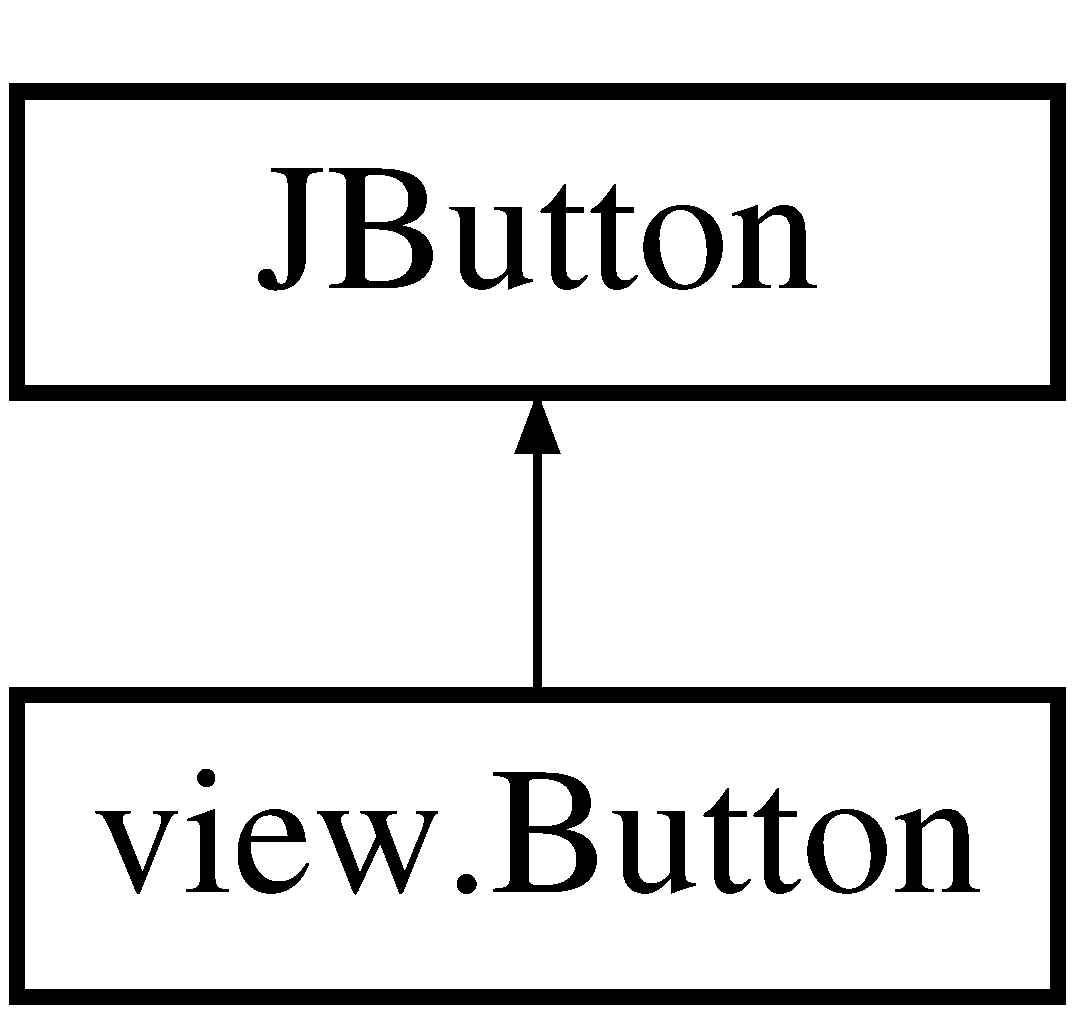
\includegraphics[height=2.000000cm]{classview_1_1_button}
\end{center}
\end{figure}
\subsection*{Public Member Functions}
\begin{DoxyCompactItemize}
\item 
\hyperlink{classview_1_1_button_a3298559ee6a99724b641f6e743027a60}{Button} (int pos\+X, int pos\+Y)
\begin{DoxyCompactList}\small\item\em Konstruktor. \end{DoxyCompactList}\item 
int \hyperlink{classview_1_1_button_ab3134b4be47315c6778c2b9afa515cf1}{get\+Pos\+X} ()
\item 
int \hyperlink{classview_1_1_button_a92639a0395cf98c55f83a570afb9a6c0}{get\+Pos\+Y} ()
\end{DoxyCompactItemize}


\subsection{Detailed Description}
A jatektablat felepito gombokat reprezentalo osztaly. 

\begin{DoxyAuthor}{Author}
team05 
\end{DoxyAuthor}


\subsection{Constructor \& Destructor Documentation}
\hypertarget{classview_1_1_button_a3298559ee6a99724b641f6e743027a60}{}\index{view\+::\+Button@{view\+::\+Button}!Button@{Button}}
\index{Button@{Button}!view\+::\+Button@{view\+::\+Button}}
\subsubsection[{Button}]{\setlength{\rightskip}{0pt plus 5cm}view.\+Button.\+Button (
\begin{DoxyParamCaption}
\item[{int}]{pos\+X, }
\item[{int}]{pos\+Y}
\end{DoxyParamCaption}
)}\label{classview_1_1_button_a3298559ee6a99724b641f6e743027a60}


Konstruktor. 


\begin{DoxyParams}{Parameters}
{\em pos\+X} & \\
\hline
{\em pos\+Y} & \\
\hline
\end{DoxyParams}


\subsection{Member Function Documentation}
\hypertarget{classview_1_1_button_ab3134b4be47315c6778c2b9afa515cf1}{}\index{view\+::\+Button@{view\+::\+Button}!get\+Pos\+X@{get\+Pos\+X}}
\index{get\+Pos\+X@{get\+Pos\+X}!view\+::\+Button@{view\+::\+Button}}
\subsubsection[{get\+Pos\+X}]{\setlength{\rightskip}{0pt plus 5cm}int view.\+Button.\+get\+Pos\+X (
\begin{DoxyParamCaption}
{}
\end{DoxyParamCaption}
)}\label{classview_1_1_button_ab3134b4be47315c6778c2b9afa515cf1}
\begin{DoxyReturn}{Returns}
int -\/ X koord 
\end{DoxyReturn}
\hypertarget{classview_1_1_button_a92639a0395cf98c55f83a570afb9a6c0}{}\index{view\+::\+Button@{view\+::\+Button}!get\+Pos\+Y@{get\+Pos\+Y}}
\index{get\+Pos\+Y@{get\+Pos\+Y}!view\+::\+Button@{view\+::\+Button}}
\subsubsection[{get\+Pos\+Y}]{\setlength{\rightskip}{0pt plus 5cm}int view.\+Button.\+get\+Pos\+Y (
\begin{DoxyParamCaption}
{}
\end{DoxyParamCaption}
)}\label{classview_1_1_button_a92639a0395cf98c55f83a570afb9a6c0}
\begin{DoxyReturn}{Returns}
int -\/ Y koord 
\end{DoxyReturn}


The documentation for this class was generated from the following file\+:\begin{DoxyCompactItemize}
\item 
C\+:/\+Users/Ádám/\+Desktop/2/checkers/src/view/Button.\+java\end{DoxyCompactItemize}

\hypertarget{classcontroller_1_1_checkers_controller}{}\section{controller.\+Checkers\+Controller Class Reference}
\label{classcontroller_1_1_checkers_controller}\index{controller.\+Checkers\+Controller@{controller.\+Checkers\+Controller}}


A modellt es a nezetet osszekoto osztaly.  


Inheritance diagram for controller.\+Checkers\+Controller\+:\begin{figure}[H]
\begin{center}
\leavevmode
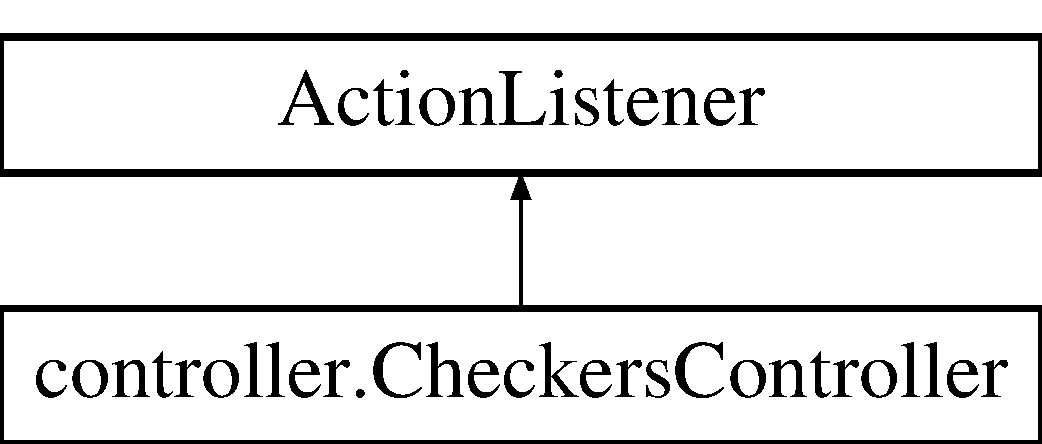
\includegraphics[height=2.000000cm]{classcontroller_1_1_checkers_controller}
\end{center}
\end{figure}
\subsection*{Public Member Functions}
\begin{DoxyCompactItemize}
\item 
\hypertarget{classcontroller_1_1_checkers_controller_aea41f08d7c97c8b62a4758ca68e9b5eb}{}\hyperlink{classcontroller_1_1_checkers_controller_aea41f08d7c97c8b62a4758ca68e9b5eb}{Checkers\+Controller} ()\label{classcontroller_1_1_checkers_controller_aea41f08d7c97c8b62a4758ca68e9b5eb}

\begin{DoxyCompactList}\small\item\em Konstruktor. \end{DoxyCompactList}\item 
void \hyperlink{classcontroller_1_1_checkers_controller_a4c010cb052e90666cc44bea483f135a3}{action\+Performed} (java.\+awt.\+event.\+Action\+Event e)
\begin{DoxyCompactList}\small\item\em Esemenyt var parameterul. Aszerint jar el, hogy a jatekter mely reszere kattintottunk. \end{DoxyCompactList}\item 
void \hyperlink{classcontroller_1_1_checkers_controller_ab93b5e14e8fb548059fe78dd90722717}{capture} (\hyperlink{classview_1_1_button}{Button} bu)
\begin{DoxyCompactList}\small\item\em A parameterul kapott gomb ut egy ellenfel babut. Az ellenfelet eltuntetni, a jatekost leptetni kell. \end{DoxyCompactList}\item 
void \hyperlink{classcontroller_1_1_checkers_controller_a5ccd4ef2422c2e730ae8dcee65e67837}{become\+Queen} (\hyperlink{classview_1_1_button}{Button} bu)
\begin{DoxyCompactList}\small\item\em A jatekos atert az ellenfel alapvonalara, kiralynove valtozik, innentol hatrafele is lephet. \end{DoxyCompactList}\item 
void \hyperlink{classcontroller_1_1_checkers_controller_a285e632cf4e9f9e1775e406fcfe8d1f9}{add\+Model} (\hyperlink{classmodel_1_1_checkers_model}{Checkers\+Model} m)
\begin{DoxyCompactList}\small\item\em Osszekottetes megteremtese a modellel. \end{DoxyCompactList}\item 
void \hyperlink{classcontroller_1_1_checkers_controller_a4682a3b99c443dbad6662b1795cde1b9}{add\+View} (\hyperlink{classview_1_1_checkers_view}{Checkers\+View} v)
\begin{DoxyCompactList}\small\item\em Osszekottetes megteremtese a nezettel. \end{DoxyCompactList}\end{DoxyCompactItemize}


\subsection{Detailed Description}
A modellt es a nezetet osszekoto osztaly. 

\begin{DoxyAuthor}{Author}
team05 
\end{DoxyAuthor}


\subsection{Member Function Documentation}
\hypertarget{classcontroller_1_1_checkers_controller_a4c010cb052e90666cc44bea483f135a3}{}\index{controller\+::\+Checkers\+Controller@{controller\+::\+Checkers\+Controller}!action\+Performed@{action\+Performed}}
\index{action\+Performed@{action\+Performed}!controller\+::\+Checkers\+Controller@{controller\+::\+Checkers\+Controller}}
\subsubsection[{action\+Performed}]{\setlength{\rightskip}{0pt plus 5cm}void controller.\+Checkers\+Controller.\+action\+Performed (
\begin{DoxyParamCaption}
\item[{java.\+awt.\+event.\+Action\+Event}]{e}
\end{DoxyParamCaption}
)}\label{classcontroller_1_1_checkers_controller_a4c010cb052e90666cc44bea483f135a3}


Esemenyt var parameterul. Aszerint jar el, hogy a jatekter mely reszere kattintottunk. 


\begin{DoxyParams}{Parameters}
{\em e} & \\
\hline
\end{DoxyParams}
\hypertarget{classcontroller_1_1_checkers_controller_a285e632cf4e9f9e1775e406fcfe8d1f9}{}\index{controller\+::\+Checkers\+Controller@{controller\+::\+Checkers\+Controller}!add\+Model@{add\+Model}}
\index{add\+Model@{add\+Model}!controller\+::\+Checkers\+Controller@{controller\+::\+Checkers\+Controller}}
\subsubsection[{add\+Model}]{\setlength{\rightskip}{0pt plus 5cm}void controller.\+Checkers\+Controller.\+add\+Model (
\begin{DoxyParamCaption}
\item[{{\bf Checkers\+Model}}]{m}
\end{DoxyParamCaption}
)}\label{classcontroller_1_1_checkers_controller_a285e632cf4e9f9e1775e406fcfe8d1f9}


Osszekottetes megteremtese a modellel. 


\begin{DoxyParams}{Parameters}
{\em m} & \\
\hline
\end{DoxyParams}
\hypertarget{classcontroller_1_1_checkers_controller_a4682a3b99c443dbad6662b1795cde1b9}{}\index{controller\+::\+Checkers\+Controller@{controller\+::\+Checkers\+Controller}!add\+View@{add\+View}}
\index{add\+View@{add\+View}!controller\+::\+Checkers\+Controller@{controller\+::\+Checkers\+Controller}}
\subsubsection[{add\+View}]{\setlength{\rightskip}{0pt plus 5cm}void controller.\+Checkers\+Controller.\+add\+View (
\begin{DoxyParamCaption}
\item[{{\bf Checkers\+View}}]{v}
\end{DoxyParamCaption}
)}\label{classcontroller_1_1_checkers_controller_a4682a3b99c443dbad6662b1795cde1b9}


Osszekottetes megteremtese a nezettel. 


\begin{DoxyParams}{Parameters}
{\em v} & \\
\hline
\end{DoxyParams}
\hypertarget{classcontroller_1_1_checkers_controller_a5ccd4ef2422c2e730ae8dcee65e67837}{}\index{controller\+::\+Checkers\+Controller@{controller\+::\+Checkers\+Controller}!become\+Queen@{become\+Queen}}
\index{become\+Queen@{become\+Queen}!controller\+::\+Checkers\+Controller@{controller\+::\+Checkers\+Controller}}
\subsubsection[{become\+Queen}]{\setlength{\rightskip}{0pt plus 5cm}void controller.\+Checkers\+Controller.\+become\+Queen (
\begin{DoxyParamCaption}
\item[{{\bf Button}}]{bu}
\end{DoxyParamCaption}
)}\label{classcontroller_1_1_checkers_controller_a5ccd4ef2422c2e730ae8dcee65e67837}


A jatekos atert az ellenfel alapvonalara, kiralynove valtozik, innentol hatrafele is lephet. 


\begin{DoxyParams}{Parameters}
{\em bu} & \\
\hline
\end{DoxyParams}
\hypertarget{classcontroller_1_1_checkers_controller_ab93b5e14e8fb548059fe78dd90722717}{}\index{controller\+::\+Checkers\+Controller@{controller\+::\+Checkers\+Controller}!capture@{capture}}
\index{capture@{capture}!controller\+::\+Checkers\+Controller@{controller\+::\+Checkers\+Controller}}
\subsubsection[{capture}]{\setlength{\rightskip}{0pt plus 5cm}void controller.\+Checkers\+Controller.\+capture (
\begin{DoxyParamCaption}
\item[{{\bf Button}}]{bu}
\end{DoxyParamCaption}
)}\label{classcontroller_1_1_checkers_controller_ab93b5e14e8fb548059fe78dd90722717}


A parameterul kapott gomb ut egy ellenfel babut. Az ellenfelet eltuntetni, a jatekost leptetni kell. 


\begin{DoxyParams}{Parameters}
{\em bu} & \\
\hline
\end{DoxyParams}


The documentation for this class was generated from the following file\+:\begin{DoxyCompactItemize}
\item 
C\+:/\+Users/Ádám/\+Desktop/2/checkers/src/controller/Checkers\+Controller.\+java\end{DoxyCompactItemize}

\hypertarget{classmodel_1_1_checkers_figure}{}\section{model.\+Checkers\+Figure Class Reference}
\label{classmodel_1_1_checkers_figure}\index{model.\+Checkers\+Figure@{model.\+Checkers\+Figure}}


A dama jatek figuraja.  


Inheritance diagram for model.\+Checkers\+Figure\+:\begin{figure}[H]
\begin{center}
\leavevmode
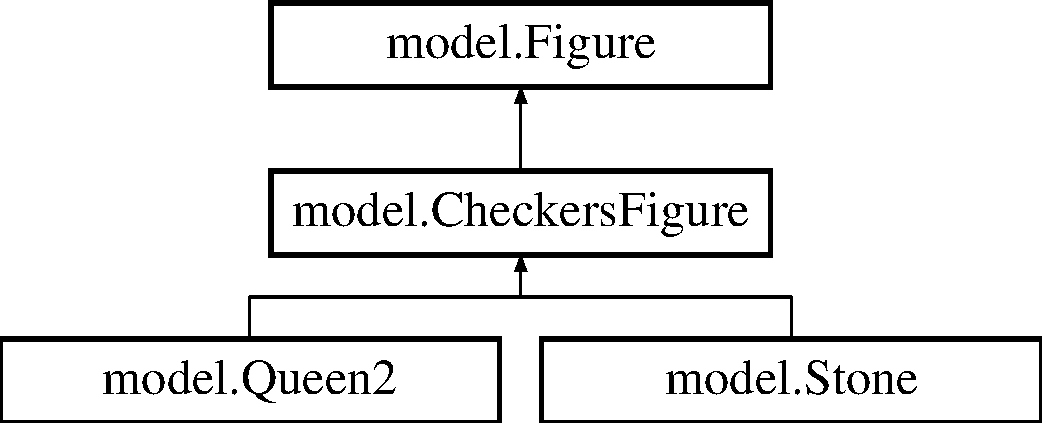
\includegraphics[height=3.000000cm]{classmodel_1_1_checkers_figure}
\end{center}
\end{figure}
\subsection*{Public Member Functions}
\begin{DoxyCompactItemize}
\item 
\hyperlink{classmodel_1_1_checkers_figure_a0895c32601056df41de919c5e20b76ab}{Checkers\+Figure} (int pos\+X, int pos\+Y, boolean dark)
\begin{DoxyCompactList}\small\item\em Konstruktor. \end{DoxyCompactList}\item 
\hypertarget{classmodel_1_1_checkers_figure_a8430b4bc382aa2e8b9d09511552490f8}{}boolean {\bfseries can\+Move\+To} (int x, int y)\label{classmodel_1_1_checkers_figure_a8430b4bc382aa2e8b9d09511552490f8}

\end{DoxyCompactItemize}


\subsection{Detailed Description}
A dama jatek figuraja. 

\begin{DoxyAuthor}{Author}
team05 
\end{DoxyAuthor}


\subsection{Constructor \& Destructor Documentation}
\hypertarget{classmodel_1_1_checkers_figure_a0895c32601056df41de919c5e20b76ab}{}\index{model\+::\+Checkers\+Figure@{model\+::\+Checkers\+Figure}!Checkers\+Figure@{Checkers\+Figure}}
\index{Checkers\+Figure@{Checkers\+Figure}!model\+::\+Checkers\+Figure@{model\+::\+Checkers\+Figure}}
\subsubsection[{Checkers\+Figure}]{\setlength{\rightskip}{0pt plus 5cm}model.\+Checkers\+Figure.\+Checkers\+Figure (
\begin{DoxyParamCaption}
\item[{int}]{pos\+X, }
\item[{int}]{pos\+Y, }
\item[{boolean}]{dark}
\end{DoxyParamCaption}
)}\label{classmodel_1_1_checkers_figure_a0895c32601056df41de919c5e20b76ab}


Konstruktor. 


\begin{DoxyParams}{Parameters}
{\em pos\+X} & \\
\hline
{\em pos\+Y} & \\
\hline
{\em dark} & \\
\hline
\end{DoxyParams}


The documentation for this class was generated from the following file\+:\begin{DoxyCompactItemize}
\item 
C\+:/\+Users/Ádám/\+Desktop/2/checkers/src/model/Checkers\+Figure.\+java\end{DoxyCompactItemize}

\hypertarget{classmodel_1_1_checkers_model}{}\section{model.\+Checkers\+Model Class Reference}
\label{classmodel_1_1_checkers_model}\index{model.\+Checkers\+Model@{model.\+Checkers\+Model}}


A tabla modellje. Logikailag itt zajlik a jatek.  


Inheritance diagram for model.\+Checkers\+Model\+:\begin{figure}[H]
\begin{center}
\leavevmode
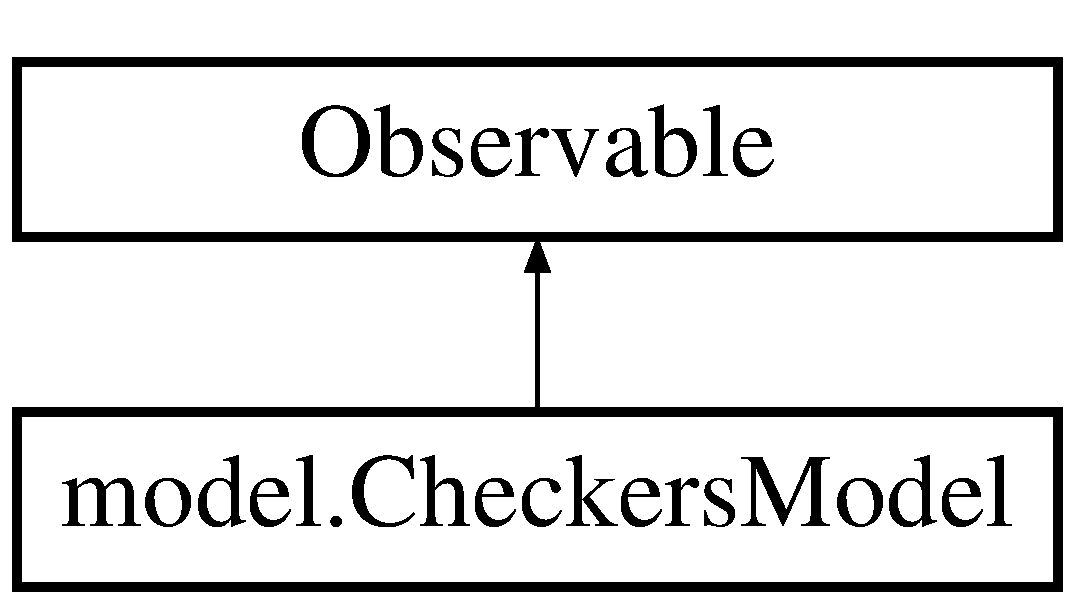
\includegraphics[height=2.000000cm]{classmodel_1_1_checkers_model}
\end{center}
\end{figure}
\subsection*{Public Member Functions}
\begin{DoxyCompactItemize}
\item 
\hypertarget{classmodel_1_1_checkers_model_ac6911ccd3b1d3718db06fd8ea7f2d7b3}{}void \hyperlink{classmodel_1_1_checkers_model_ac6911ccd3b1d3718db06fd8ea7f2d7b3}{set\+Default\+Figures} ()\label{classmodel_1_1_checkers_model_ac6911ccd3b1d3718db06fd8ea7f2d7b3}

\begin{DoxyCompactList}\small\item\em A standard jatekosok betoltese. \end{DoxyCompactList}\item 
\hyperlink{classmodel_1_1_checkers_figure}{Checkers\+Figure} \hyperlink{classmodel_1_1_checkers_model_a3c802fe132a08baddf712e09df96cab9}{get\+Figure} (int x, int y)
\begin{DoxyCompactList}\small\item\em Adott poziciorol visszaadja a babu objektumot. \end{DoxyCompactList}\item 
List$<$ \hyperlink{classmodel_1_1_pair}{Pair} $>$ \hyperlink{classmodel_1_1_checkers_model_a5bf2d3775839b95e7f13cf3e765b6981}{set\+Can\+Move\+To} (int x, int y)
\begin{DoxyCompactList}\small\item\em Visszaadja azon poziciok listajat, ahova lephetunk. \end{DoxyCompactList}\item 
void \hyperlink{classmodel_1_1_checkers_model_ad36574e98ce2f7b1983d25c376e0a3e6}{set\+Figure} (int x, int y, \hyperlink{classmodel_1_1_checkers_figure}{Checkers\+Figure} f)
\begin{DoxyCompactList}\small\item\em A tablat reprezentalo matrix adott poziciojat beallitja a parameterul kapott figuranak. \end{DoxyCompactList}\item 
boolean \hyperlink{classmodel_1_1_checkers_model_a2825ba09fc35c7fa69c0ab470a32c0db}{is\+Game\+Over} (boolean dark)
\begin{DoxyCompactList}\small\item\em A jatek veget figyelo fuggveny. \end{DoxyCompactList}\item 
boolean \hyperlink{classmodel_1_1_checkers_model_a3390a48c6e78518edd28532969fc46d6}{stone\+Can\+Move} (int from\+X, int from\+Y, int to\+X, int to\+Y)
\begin{DoxyCompactList}\small\item\em Honnan hova lephetunk figyeleset vegzo fuggeny (alapbabuval). \end{DoxyCompactList}\item 
boolean \hyperlink{classmodel_1_1_checkers_model_a598d81ff2ad93c90dfa1cf3bcad5422c}{queen\+Can\+Move} (int from\+X, int from\+Y, int to\+X, int to\+Y)
\begin{DoxyCompactList}\small\item\em Honnan hova lephetunk figyeleset vegzo fuggeny (kiralynovel). \end{DoxyCompactList}\item 
boolean \hyperlink{classmodel_1_1_checkers_model_aaafda9b9ae1510b65a7c1a576255a5b0}{stone\+Can\+Capture} (int from\+X, int from\+Y, int to\+X, int to\+Y)
\begin{DoxyCompactList}\small\item\em Azt figyeli, hogy le tudunk e venni az ellenfel jatekosai kozul. (alapbabuval) \end{DoxyCompactList}\item 
boolean \hyperlink{classmodel_1_1_checkers_model_ab9109be8e090812d614b3aa9f8cf3a7b}{queen\+Can\+Capture} (int from\+X, int from\+Y, int to\+X, int to\+Y)
\begin{DoxyCompactList}\small\item\em Azt figyeli, hogy le tudunk e venni az ellenfel jatekosai kozul. (kiralynovel) \end{DoxyCompactList}\end{DoxyCompactItemize}


\subsection{Detailed Description}
A tabla modellje. Logikailag itt zajlik a jatek. 

\begin{DoxyAuthor}{Author}
team05 
\end{DoxyAuthor}


\subsection{Member Function Documentation}
\hypertarget{classmodel_1_1_checkers_model_a3c802fe132a08baddf712e09df96cab9}{}\index{model\+::\+Checkers\+Model@{model\+::\+Checkers\+Model}!get\+Figure@{get\+Figure}}
\index{get\+Figure@{get\+Figure}!model\+::\+Checkers\+Model@{model\+::\+Checkers\+Model}}
\subsubsection[{get\+Figure}]{\setlength{\rightskip}{0pt plus 5cm}{\bf Checkers\+Figure} model.\+Checkers\+Model.\+get\+Figure (
\begin{DoxyParamCaption}
\item[{int}]{x, }
\item[{int}]{y}
\end{DoxyParamCaption}
)}\label{classmodel_1_1_checkers_model_a3c802fe132a08baddf712e09df96cab9}


Adott poziciorol visszaadja a babu objektumot. 


\begin{DoxyParams}{Parameters}
{\em x} & \\
\hline
{\em y} & \\
\hline
\end{DoxyParams}
\begin{DoxyReturn}{Returns}
\hyperlink{classmodel_1_1_checkers_figure}{Checkers\+Figure} 
\end{DoxyReturn}
\hypertarget{classmodel_1_1_checkers_model_a2825ba09fc35c7fa69c0ab470a32c0db}{}\index{model\+::\+Checkers\+Model@{model\+::\+Checkers\+Model}!is\+Game\+Over@{is\+Game\+Over}}
\index{is\+Game\+Over@{is\+Game\+Over}!model\+::\+Checkers\+Model@{model\+::\+Checkers\+Model}}
\subsubsection[{is\+Game\+Over}]{\setlength{\rightskip}{0pt plus 5cm}boolean model.\+Checkers\+Model.\+is\+Game\+Over (
\begin{DoxyParamCaption}
\item[{boolean}]{dark}
\end{DoxyParamCaption}
)}\label{classmodel_1_1_checkers_model_a2825ba09fc35c7fa69c0ab470a32c0db}


A jatek veget figyelo fuggveny. 


\begin{DoxyParams}{Parameters}
{\em dark} & \\
\hline
\end{DoxyParams}
\begin{DoxyReturn}{Returns}
boolean 
\end{DoxyReturn}
\hypertarget{classmodel_1_1_checkers_model_ab9109be8e090812d614b3aa9f8cf3a7b}{}\index{model\+::\+Checkers\+Model@{model\+::\+Checkers\+Model}!queen\+Can\+Capture@{queen\+Can\+Capture}}
\index{queen\+Can\+Capture@{queen\+Can\+Capture}!model\+::\+Checkers\+Model@{model\+::\+Checkers\+Model}}
\subsubsection[{queen\+Can\+Capture}]{\setlength{\rightskip}{0pt plus 5cm}boolean model.\+Checkers\+Model.\+queen\+Can\+Capture (
\begin{DoxyParamCaption}
\item[{int}]{from\+X, }
\item[{int}]{from\+Y, }
\item[{int}]{to\+X, }
\item[{int}]{to\+Y}
\end{DoxyParamCaption}
)}\label{classmodel_1_1_checkers_model_ab9109be8e090812d614b3aa9f8cf3a7b}


Azt figyeli, hogy le tudunk e venni az ellenfel jatekosai kozul. (kiralynovel) 


\begin{DoxyParams}{Parameters}
{\em from\+X} & \\
\hline
{\em from\+Y} & \\
\hline
{\em to\+X} & \\
\hline
{\em to\+Y} & \\
\hline
\end{DoxyParams}
\begin{DoxyReturn}{Returns}
bool 
\end{DoxyReturn}
\hypertarget{classmodel_1_1_checkers_model_a598d81ff2ad93c90dfa1cf3bcad5422c}{}\index{model\+::\+Checkers\+Model@{model\+::\+Checkers\+Model}!queen\+Can\+Move@{queen\+Can\+Move}}
\index{queen\+Can\+Move@{queen\+Can\+Move}!model\+::\+Checkers\+Model@{model\+::\+Checkers\+Model}}
\subsubsection[{queen\+Can\+Move}]{\setlength{\rightskip}{0pt plus 5cm}boolean model.\+Checkers\+Model.\+queen\+Can\+Move (
\begin{DoxyParamCaption}
\item[{int}]{from\+X, }
\item[{int}]{from\+Y, }
\item[{int}]{to\+X, }
\item[{int}]{to\+Y}
\end{DoxyParamCaption}
)}\label{classmodel_1_1_checkers_model_a598d81ff2ad93c90dfa1cf3bcad5422c}


Honnan hova lephetunk figyeleset vegzo fuggeny (kiralynovel). 


\begin{DoxyParams}{Parameters}
{\em from\+X} & \\
\hline
{\em from\+Y} & \\
\hline
{\em to\+X} & \\
\hline
{\em to\+Y} & \\
\hline
\end{DoxyParams}
\begin{DoxyReturn}{Returns}
boolean 
\end{DoxyReturn}
\hypertarget{classmodel_1_1_checkers_model_a5bf2d3775839b95e7f13cf3e765b6981}{}\index{model\+::\+Checkers\+Model@{model\+::\+Checkers\+Model}!set\+Can\+Move\+To@{set\+Can\+Move\+To}}
\index{set\+Can\+Move\+To@{set\+Can\+Move\+To}!model\+::\+Checkers\+Model@{model\+::\+Checkers\+Model}}
\subsubsection[{set\+Can\+Move\+To}]{\setlength{\rightskip}{0pt plus 5cm}List$<${\bf Pair}$>$ model.\+Checkers\+Model.\+set\+Can\+Move\+To (
\begin{DoxyParamCaption}
\item[{int}]{x, }
\item[{int}]{y}
\end{DoxyParamCaption}
)}\label{classmodel_1_1_checkers_model_a5bf2d3775839b95e7f13cf3e765b6981}


Visszaadja azon poziciok listajat, ahova lephetunk. 


\begin{DoxyParams}{Parameters}
{\em x} & \\
\hline
{\em y} & \\
\hline
\end{DoxyParams}
\begin{DoxyReturn}{Returns}
List -\/ azon poziciok listaja, ahova lephetunk 
\end{DoxyReturn}
\hypertarget{classmodel_1_1_checkers_model_ad36574e98ce2f7b1983d25c376e0a3e6}{}\index{model\+::\+Checkers\+Model@{model\+::\+Checkers\+Model}!set\+Figure@{set\+Figure}}
\index{set\+Figure@{set\+Figure}!model\+::\+Checkers\+Model@{model\+::\+Checkers\+Model}}
\subsubsection[{set\+Figure}]{\setlength{\rightskip}{0pt plus 5cm}void model.\+Checkers\+Model.\+set\+Figure (
\begin{DoxyParamCaption}
\item[{int}]{x, }
\item[{int}]{y, }
\item[{{\bf Checkers\+Figure}}]{f}
\end{DoxyParamCaption}
)}\label{classmodel_1_1_checkers_model_ad36574e98ce2f7b1983d25c376e0a3e6}


A tablat reprezentalo matrix adott poziciojat beallitja a parameterul kapott figuranak. 


\begin{DoxyParams}{Parameters}
{\em x} & \\
\hline
{\em y} & \\
\hline
{\em f} & \\
\hline
\end{DoxyParams}
\hypertarget{classmodel_1_1_checkers_model_aaafda9b9ae1510b65a7c1a576255a5b0}{}\index{model\+::\+Checkers\+Model@{model\+::\+Checkers\+Model}!stone\+Can\+Capture@{stone\+Can\+Capture}}
\index{stone\+Can\+Capture@{stone\+Can\+Capture}!model\+::\+Checkers\+Model@{model\+::\+Checkers\+Model}}
\subsubsection[{stone\+Can\+Capture}]{\setlength{\rightskip}{0pt plus 5cm}boolean model.\+Checkers\+Model.\+stone\+Can\+Capture (
\begin{DoxyParamCaption}
\item[{int}]{from\+X, }
\item[{int}]{from\+Y, }
\item[{int}]{to\+X, }
\item[{int}]{to\+Y}
\end{DoxyParamCaption}
)}\label{classmodel_1_1_checkers_model_aaafda9b9ae1510b65a7c1a576255a5b0}


Azt figyeli, hogy le tudunk e venni az ellenfel jatekosai kozul. (alapbabuval) 


\begin{DoxyParams}{Parameters}
{\em from\+X} & \\
\hline
{\em from\+Y} & \\
\hline
{\em to\+X} & \\
\hline
{\em to\+Y} & \\
\hline
\end{DoxyParams}
\begin{DoxyReturn}{Returns}
boolean 
\end{DoxyReturn}
\hypertarget{classmodel_1_1_checkers_model_a3390a48c6e78518edd28532969fc46d6}{}\index{model\+::\+Checkers\+Model@{model\+::\+Checkers\+Model}!stone\+Can\+Move@{stone\+Can\+Move}}
\index{stone\+Can\+Move@{stone\+Can\+Move}!model\+::\+Checkers\+Model@{model\+::\+Checkers\+Model}}
\subsubsection[{stone\+Can\+Move}]{\setlength{\rightskip}{0pt plus 5cm}boolean model.\+Checkers\+Model.\+stone\+Can\+Move (
\begin{DoxyParamCaption}
\item[{int}]{from\+X, }
\item[{int}]{from\+Y, }
\item[{int}]{to\+X, }
\item[{int}]{to\+Y}
\end{DoxyParamCaption}
)}\label{classmodel_1_1_checkers_model_a3390a48c6e78518edd28532969fc46d6}


Honnan hova lephetunk figyeleset vegzo fuggeny (alapbabuval). 


\begin{DoxyParams}{Parameters}
{\em from\+X} & \\
\hline
{\em from\+Y} & \\
\hline
{\em to\+X} & \\
\hline
{\em to\+Y} & \\
\hline
\end{DoxyParams}
\begin{DoxyReturn}{Returns}
boolean 
\end{DoxyReturn}


The documentation for this class was generated from the following file\+:\begin{DoxyCompactItemize}
\item 
C\+:/\+Users/Ádám/\+Desktop/2/checkers/src/model/Checkers\+Model.\+java\end{DoxyCompactItemize}

\hypertarget{classview_1_1_checkers_view}{}\section{view.\+Checkers\+View Class Reference}
\label{classview_1_1_checkers_view}\index{view.\+Checkers\+View@{view.\+Checkers\+View}}


A dama jatek megjeleniteset vegzo osztaly.  


Inheritance diagram for view.\+Checkers\+View\+:\begin{figure}[H]
\begin{center}
\leavevmode
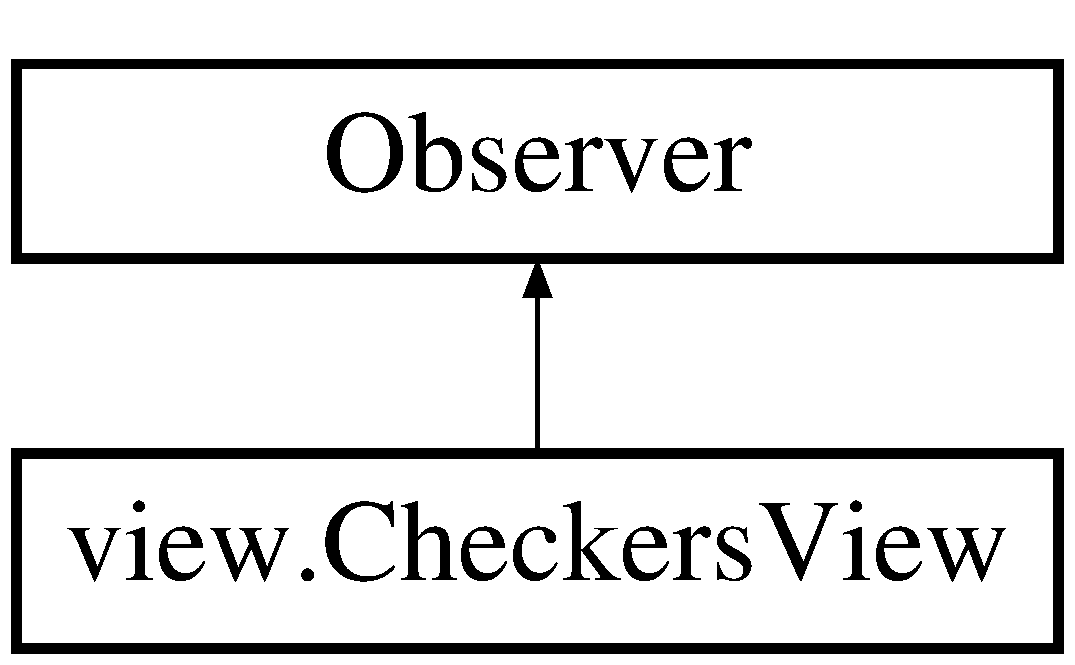
\includegraphics[height=2.000000cm]{classview_1_1_checkers_view}
\end{center}
\end{figure}
\subsection*{Classes}
\begin{DoxyCompactItemize}
\item 
class {\bfseries Close\+Listener}
\begin{DoxyCompactList}\small\item\em Ablak bezaras esemenyt figyelo osztaly. \end{DoxyCompactList}\end{DoxyCompactItemize}
\subsection*{Public Member Functions}
\begin{DoxyCompactItemize}
\item 
\hypertarget{classview_1_1_checkers_view_a32d5da333ffe78031b1717b10a583d01}{}void \hyperlink{classview_1_1_checkers_view_a32d5da333ffe78031b1717b10a583d01}{add\+Controller} (Action\+Listener controller)\label{classview_1_1_checkers_view_a32d5da333ffe78031b1717b10a583d01}

\begin{DoxyCompactList}\small\item\em Eseménykezelok hozzaadasa a gombokhoz, tablahoz. \end{DoxyCompactList}\item 
\hypertarget{classview_1_1_checkers_view_a5ed677cd4f78c6168bebbe4bf311bff5}{}void \hyperlink{classview_1_1_checkers_view_a5ed677cd4f78c6168bebbe4bf311bff5}{go\+To\+Menu} ()\label{classview_1_1_checkers_view_a5ed677cd4f78c6168bebbe4bf311bff5}

\begin{DoxyCompactList}\small\item\em Vissza a menube gomb mukodtetese. \end{DoxyCompactList}\item 
void \hyperlink{classview_1_1_checkers_view_a68fe3b1f0a965c499d06c2c0ac4364bf}{set\+Unselected} (\hyperlink{classview_1_1_button}{Button} bu)
\begin{DoxyCompactList}\small\item\em Vissza allitjuk a korabbi szinre a gomb szinet, \char`\"{}nincs kijelölve\char`\"{}. \end{DoxyCompactList}\item 
\hypertarget{classview_1_1_checkers_view_a8a5602a18f240d3262866c354995c4e5}{}void \hyperlink{classview_1_1_checkers_view_a8a5602a18f240d3262866c354995c4e5}{reset\+Back\+Grounds} ()\label{classview_1_1_checkers_view_a8a5602a18f240d3262866c354995c4e5}

\begin{DoxyCompactList}\small\item\em Visszaallitja a tablat az eredeti allapotba. \end{DoxyCompactList}\item 
void \hyperlink{classview_1_1_checkers_view_a6aba0221126505b6647d0e3265bd1d93}{set\+Queen} (int x, int y, boolean dark)
\begin{DoxyCompactList}\small\item\em Stone-\/bol kiralyno (dama). \end{DoxyCompactList}\item 
void \hyperlink{classview_1_1_checkers_view_a7ed18b58b6aad5b1aafe96c26e5941ca}{set\+Red} (\hyperlink{classview_1_1_button}{Button} bu)
\begin{DoxyCompactList}\small\item\em Beállítja a parameterkent kapott gomb szinet pirosra. \end{DoxyCompactList}\item 
void \hyperlink{classview_1_1_checkers_view_a0fb36a93cfc88b8a844df820fdf0dc11}{set\+Blue} (\hyperlink{classview_1_1_button}{Button} bu)
\begin{DoxyCompactList}\small\item\em Beállítja a parameteskent kapott gomb szinet kekre. \end{DoxyCompactList}\item 
\hyperlink{classview_1_1_button}{Button} \hyperlink{classview_1_1_checkers_view_a0cec5bc3e85bb43da33dc98bb84cb618}{get\+Button\+At} (int x, int y)
\begin{DoxyCompactList}\small\item\em Visszadjuk a parameterkent kapott pozicioban talalhato gombot. \end{DoxyCompactList}\item 
Icon \hyperlink{classview_1_1_checkers_view_a4193841f5fe3bf1a4345d947630eac82}{get\+Icon} (int x, int y)
\begin{DoxyCompactList}\small\item\em Visszaadja az adott pozicion talalhato gomb ikonjat. \end{DoxyCompactList}\item 
void \hyperlink{classview_1_1_checkers_view_aaa2497d67e7b4ff8def470ce78068ff7}{set\+Icon} (int x, int y, Icon icon)
\begin{DoxyCompactList}\small\item\em Az adott pozicion levo gombnak a parameterul kapott ikont adjuk kepkent. \end{DoxyCompactList}\item 
void \hyperlink{classview_1_1_checkers_view_aba0423decf4638146a48f9ec40a9464c}{game\+Over} (boolean dark)
\begin{DoxyCompactList}\small\item\em Jatek veget jelzo ablak. \end{DoxyCompactList}\item 
void \hyperlink{classview_1_1_checkers_view_a7a71823b8690bb5cadcfe1fa530b2e00}{set\+Label} (boolean dark)
\begin{DoxyCompactList}\small\item\em A kovetkezo jatekos jelzesere szolgalo kiiras. \end{DoxyCompactList}\item 
void \hyperlink{classview_1_1_checkers_view_a5a4d8d0eac9b0d605821d1826718aaa2}{update} (Observable o, Object arg)
\begin{DoxyCompactList}\small\item\em Kotelezoen feluldefinialando fuggveny. \end{DoxyCompactList}\end{DoxyCompactItemize}


\subsection{Detailed Description}
A dama jatek megjeleniteset vegzo osztaly. 

\begin{DoxyAuthor}{Author}
team05 
\end{DoxyAuthor}


\subsection{Member Function Documentation}
\hypertarget{classview_1_1_checkers_view_aba0423decf4638146a48f9ec40a9464c}{}\index{view\+::\+Checkers\+View@{view\+::\+Checkers\+View}!game\+Over@{game\+Over}}
\index{game\+Over@{game\+Over}!view\+::\+Checkers\+View@{view\+::\+Checkers\+View}}
\subsubsection[{game\+Over}]{\setlength{\rightskip}{0pt plus 5cm}void view.\+Checkers\+View.\+game\+Over (
\begin{DoxyParamCaption}
\item[{boolean}]{dark}
\end{DoxyParamCaption}
)}\label{classview_1_1_checkers_view_aba0423decf4638146a48f9ec40a9464c}


Jatek veget jelzo ablak. 


\begin{DoxyParams}{Parameters}
{\em dark} & \\
\hline
\end{DoxyParams}
\hypertarget{classview_1_1_checkers_view_a0cec5bc3e85bb43da33dc98bb84cb618}{}\index{view\+::\+Checkers\+View@{view\+::\+Checkers\+View}!get\+Button\+At@{get\+Button\+At}}
\index{get\+Button\+At@{get\+Button\+At}!view\+::\+Checkers\+View@{view\+::\+Checkers\+View}}
\subsubsection[{get\+Button\+At}]{\setlength{\rightskip}{0pt plus 5cm}{\bf Button} view.\+Checkers\+View.\+get\+Button\+At (
\begin{DoxyParamCaption}
\item[{int}]{x, }
\item[{int}]{y}
\end{DoxyParamCaption}
)}\label{classview_1_1_checkers_view_a0cec5bc3e85bb43da33dc98bb84cb618}


Visszadjuk a parameterkent kapott pozicioban talalhato gombot. 


\begin{DoxyParams}{Parameters}
{\em x} & \\
\hline
{\em y} & \\
\hline
\end{DoxyParams}
\begin{DoxyReturn}{Returns}
button 
\end{DoxyReturn}
\hypertarget{classview_1_1_checkers_view_a4193841f5fe3bf1a4345d947630eac82}{}\index{view\+::\+Checkers\+View@{view\+::\+Checkers\+View}!get\+Icon@{get\+Icon}}
\index{get\+Icon@{get\+Icon}!view\+::\+Checkers\+View@{view\+::\+Checkers\+View}}
\subsubsection[{get\+Icon}]{\setlength{\rightskip}{0pt plus 5cm}Icon view.\+Checkers\+View.\+get\+Icon (
\begin{DoxyParamCaption}
\item[{int}]{x, }
\item[{int}]{y}
\end{DoxyParamCaption}
)}\label{classview_1_1_checkers_view_a4193841f5fe3bf1a4345d947630eac82}


Visszaadja az adott pozicion talalhato gomb ikonjat. 


\begin{DoxyParams}{Parameters}
{\em x} & \\
\hline
{\em y} & \\
\hline
\end{DoxyParams}
\begin{DoxyReturn}{Returns}
icon 
\end{DoxyReturn}
\hypertarget{classview_1_1_checkers_view_a0fb36a93cfc88b8a844df820fdf0dc11}{}\index{view\+::\+Checkers\+View@{view\+::\+Checkers\+View}!set\+Blue@{set\+Blue}}
\index{set\+Blue@{set\+Blue}!view\+::\+Checkers\+View@{view\+::\+Checkers\+View}}
\subsubsection[{set\+Blue}]{\setlength{\rightskip}{0pt plus 5cm}void view.\+Checkers\+View.\+set\+Blue (
\begin{DoxyParamCaption}
\item[{{\bf Button}}]{bu}
\end{DoxyParamCaption}
)}\label{classview_1_1_checkers_view_a0fb36a93cfc88b8a844df820fdf0dc11}


Beállítja a parameteskent kapott gomb szinet kekre. 


\begin{DoxyParams}{Parameters}
{\em bu} & \\
\hline
\end{DoxyParams}
\hypertarget{classview_1_1_checkers_view_aaa2497d67e7b4ff8def470ce78068ff7}{}\index{view\+::\+Checkers\+View@{view\+::\+Checkers\+View}!set\+Icon@{set\+Icon}}
\index{set\+Icon@{set\+Icon}!view\+::\+Checkers\+View@{view\+::\+Checkers\+View}}
\subsubsection[{set\+Icon}]{\setlength{\rightskip}{0pt plus 5cm}void view.\+Checkers\+View.\+set\+Icon (
\begin{DoxyParamCaption}
\item[{int}]{x, }
\item[{int}]{y, }
\item[{Icon}]{icon}
\end{DoxyParamCaption}
)}\label{classview_1_1_checkers_view_aaa2497d67e7b4ff8def470ce78068ff7}


Az adott pozicion levo gombnak a parameterul kapott ikont adjuk kepkent. 


\begin{DoxyParams}{Parameters}
{\em x} & \\
\hline
{\em y} & \\
\hline
{\em icon} & \\
\hline
\end{DoxyParams}
\hypertarget{classview_1_1_checkers_view_a7a71823b8690bb5cadcfe1fa530b2e00}{}\index{view\+::\+Checkers\+View@{view\+::\+Checkers\+View}!set\+Label@{set\+Label}}
\index{set\+Label@{set\+Label}!view\+::\+Checkers\+View@{view\+::\+Checkers\+View}}
\subsubsection[{set\+Label}]{\setlength{\rightskip}{0pt plus 5cm}void view.\+Checkers\+View.\+set\+Label (
\begin{DoxyParamCaption}
\item[{boolean}]{dark}
\end{DoxyParamCaption}
)}\label{classview_1_1_checkers_view_a7a71823b8690bb5cadcfe1fa530b2e00}


A kovetkezo jatekos jelzesere szolgalo kiiras. 


\begin{DoxyParams}{Parameters}
{\em dark} & \\
\hline
\end{DoxyParams}
\hypertarget{classview_1_1_checkers_view_a6aba0221126505b6647d0e3265bd1d93}{}\index{view\+::\+Checkers\+View@{view\+::\+Checkers\+View}!set\+Queen@{set\+Queen}}
\index{set\+Queen@{set\+Queen}!view\+::\+Checkers\+View@{view\+::\+Checkers\+View}}
\subsubsection[{set\+Queen}]{\setlength{\rightskip}{0pt plus 5cm}void view.\+Checkers\+View.\+set\+Queen (
\begin{DoxyParamCaption}
\item[{int}]{x, }
\item[{int}]{y, }
\item[{boolean}]{dark}
\end{DoxyParamCaption}
)}\label{classview_1_1_checkers_view_a6aba0221126505b6647d0e3265bd1d93}


Stone-\/bol kiralyno (dama). 


\begin{DoxyParams}{Parameters}
{\em x} & \\
\hline
{\em y} & \\
\hline
{\em dark} & \\
\hline
\end{DoxyParams}
\hypertarget{classview_1_1_checkers_view_a7ed18b58b6aad5b1aafe96c26e5941ca}{}\index{view\+::\+Checkers\+View@{view\+::\+Checkers\+View}!set\+Red@{set\+Red}}
\index{set\+Red@{set\+Red}!view\+::\+Checkers\+View@{view\+::\+Checkers\+View}}
\subsubsection[{set\+Red}]{\setlength{\rightskip}{0pt plus 5cm}void view.\+Checkers\+View.\+set\+Red (
\begin{DoxyParamCaption}
\item[{{\bf Button}}]{bu}
\end{DoxyParamCaption}
)}\label{classview_1_1_checkers_view_a7ed18b58b6aad5b1aafe96c26e5941ca}


Beállítja a parameterkent kapott gomb szinet pirosra. 


\begin{DoxyParams}{Parameters}
{\em bu} & \\
\hline
\end{DoxyParams}
\hypertarget{classview_1_1_checkers_view_a68fe3b1f0a965c499d06c2c0ac4364bf}{}\index{view\+::\+Checkers\+View@{view\+::\+Checkers\+View}!set\+Unselected@{set\+Unselected}}
\index{set\+Unselected@{set\+Unselected}!view\+::\+Checkers\+View@{view\+::\+Checkers\+View}}
\subsubsection[{set\+Unselected}]{\setlength{\rightskip}{0pt plus 5cm}void view.\+Checkers\+View.\+set\+Unselected (
\begin{DoxyParamCaption}
\item[{{\bf Button}}]{bu}
\end{DoxyParamCaption}
)}\label{classview_1_1_checkers_view_a68fe3b1f0a965c499d06c2c0ac4364bf}


Vissza allitjuk a korabbi szinre a gomb szinet, \char`\"{}nincs kijelölve\char`\"{}. 


\begin{DoxyParams}{Parameters}
{\em bu} & \\
\hline
\end{DoxyParams}
\hypertarget{classview_1_1_checkers_view_a5a4d8d0eac9b0d605821d1826718aaa2}{}\index{view\+::\+Checkers\+View@{view\+::\+Checkers\+View}!update@{update}}
\index{update@{update}!view\+::\+Checkers\+View@{view\+::\+Checkers\+View}}
\subsubsection[{update}]{\setlength{\rightskip}{0pt plus 5cm}void view.\+Checkers\+View.\+update (
\begin{DoxyParamCaption}
\item[{Observable}]{o, }
\item[{Object}]{arg}
\end{DoxyParamCaption}
)}\label{classview_1_1_checkers_view_a5a4d8d0eac9b0d605821d1826718aaa2}


Kotelezoen feluldefinialando fuggveny. 


\begin{DoxyParams}{Parameters}
{\em o} & \\
\hline
{\em arg} & \\
\hline
\end{DoxyParams}


The documentation for this class was generated from the following file\+:\begin{DoxyCompactItemize}
\item 
C\+:/\+Users/Ádám/\+Desktop/2/checkers/src/view/Checkers\+View.\+java\end{DoxyCompactItemize}

\hypertarget{classmodel_1_1_figure}{}\section{model.\+Figure Class Reference}
\label{classmodel_1_1_figure}\index{model.\+Figure@{model.\+Figure}}


A babut reprezentalo osztaly.  


Inheritance diagram for model.\+Figure\+:\begin{figure}[H]
\begin{center}
\leavevmode
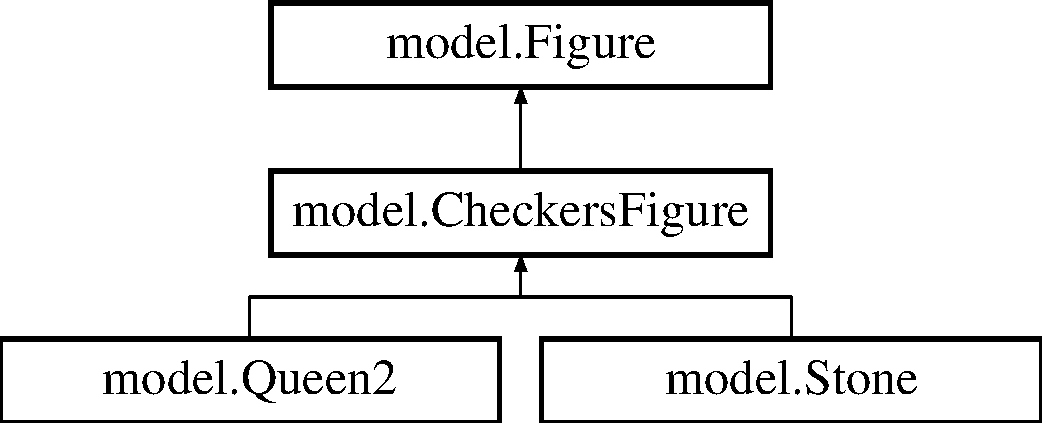
\includegraphics[height=3.000000cm]{classmodel_1_1_figure}
\end{center}
\end{figure}
\subsection*{Public Member Functions}
\begin{DoxyCompactItemize}
\item 
int \hyperlink{classmodel_1_1_figure_a358304accea622125647500452eeb17a}{get\+Pos\+X} ()
\begin{DoxyCompactList}\small\item\em Visszaadja az X koordinatat. \end{DoxyCompactList}\item 
int \hyperlink{classmodel_1_1_figure_aa777f7294810c1fb0f6d3bdb47ba6ae9}{get\+Pos\+Y} ()
\begin{DoxyCompactList}\small\item\em Visszaadja az Y koordinatat. \end{DoxyCompactList}\item 
void \hyperlink{classmodel_1_1_figure_a28566262a5ad1e7411900b167b0e9c7d}{set\+Pos\+X} (int pos\+X)
\begin{DoxyCompactList}\small\item\em Beallitja az X koordinatat. \end{DoxyCompactList}\item 
void \hyperlink{classmodel_1_1_figure_a2172418b68198d637829a8803b26ec5d}{set\+Pos\+Y} (int pos\+Y)
\begin{DoxyCompactList}\small\item\em Beallitja az Y koordinatat. \end{DoxyCompactList}\item 
boolean \hyperlink{classmodel_1_1_figure_ae0bb1f1d02bda635222b0b58a32eca53}{is\+Dark} ()
\begin{DoxyCompactList}\small\item\em Visszaadja az is\+Dark logikai valtozo erteket. \end{DoxyCompactList}\end{DoxyCompactItemize}


\subsection{Detailed Description}
A babut reprezentalo osztaly. 

\begin{DoxyAuthor}{Author}
team05 
\end{DoxyAuthor}


\subsection{Member Function Documentation}
\hypertarget{classmodel_1_1_figure_a358304accea622125647500452eeb17a}{}\index{model\+::\+Figure@{model\+::\+Figure}!get\+Pos\+X@{get\+Pos\+X}}
\index{get\+Pos\+X@{get\+Pos\+X}!model\+::\+Figure@{model\+::\+Figure}}
\subsubsection[{get\+Pos\+X}]{\setlength{\rightskip}{0pt plus 5cm}int model.\+Figure.\+get\+Pos\+X (
\begin{DoxyParamCaption}
{}
\end{DoxyParamCaption}
)}\label{classmodel_1_1_figure_a358304accea622125647500452eeb17a}


Visszaadja az X koordinatat. 

\begin{DoxyReturn}{Returns}
int 
\end{DoxyReturn}
\hypertarget{classmodel_1_1_figure_aa777f7294810c1fb0f6d3bdb47ba6ae9}{}\index{model\+::\+Figure@{model\+::\+Figure}!get\+Pos\+Y@{get\+Pos\+Y}}
\index{get\+Pos\+Y@{get\+Pos\+Y}!model\+::\+Figure@{model\+::\+Figure}}
\subsubsection[{get\+Pos\+Y}]{\setlength{\rightskip}{0pt plus 5cm}int model.\+Figure.\+get\+Pos\+Y (
\begin{DoxyParamCaption}
{}
\end{DoxyParamCaption}
)}\label{classmodel_1_1_figure_aa777f7294810c1fb0f6d3bdb47ba6ae9}


Visszaadja az Y koordinatat. 

\begin{DoxyReturn}{Returns}
int 
\end{DoxyReturn}
\hypertarget{classmodel_1_1_figure_ae0bb1f1d02bda635222b0b58a32eca53}{}\index{model\+::\+Figure@{model\+::\+Figure}!is\+Dark@{is\+Dark}}
\index{is\+Dark@{is\+Dark}!model\+::\+Figure@{model\+::\+Figure}}
\subsubsection[{is\+Dark}]{\setlength{\rightskip}{0pt plus 5cm}boolean model.\+Figure.\+is\+Dark (
\begin{DoxyParamCaption}
{}
\end{DoxyParamCaption}
)}\label{classmodel_1_1_figure_ae0bb1f1d02bda635222b0b58a32eca53}


Visszaadja az is\+Dark logikai valtozo erteket. 

\begin{DoxyReturn}{Returns}
int 
\end{DoxyReturn}
\hypertarget{classmodel_1_1_figure_a28566262a5ad1e7411900b167b0e9c7d}{}\index{model\+::\+Figure@{model\+::\+Figure}!set\+Pos\+X@{set\+Pos\+X}}
\index{set\+Pos\+X@{set\+Pos\+X}!model\+::\+Figure@{model\+::\+Figure}}
\subsubsection[{set\+Pos\+X}]{\setlength{\rightskip}{0pt plus 5cm}void model.\+Figure.\+set\+Pos\+X (
\begin{DoxyParamCaption}
\item[{int}]{pos\+X}
\end{DoxyParamCaption}
)}\label{classmodel_1_1_figure_a28566262a5ad1e7411900b167b0e9c7d}


Beallitja az X koordinatat. 

\begin{DoxyReturn}{Returns}
int 
\end{DoxyReturn}
\hypertarget{classmodel_1_1_figure_a2172418b68198d637829a8803b26ec5d}{}\index{model\+::\+Figure@{model\+::\+Figure}!set\+Pos\+Y@{set\+Pos\+Y}}
\index{set\+Pos\+Y@{set\+Pos\+Y}!model\+::\+Figure@{model\+::\+Figure}}
\subsubsection[{set\+Pos\+Y}]{\setlength{\rightskip}{0pt plus 5cm}void model.\+Figure.\+set\+Pos\+Y (
\begin{DoxyParamCaption}
\item[{int}]{pos\+Y}
\end{DoxyParamCaption}
)}\label{classmodel_1_1_figure_a2172418b68198d637829a8803b26ec5d}


Beallitja az Y koordinatat. 

\begin{DoxyReturn}{Returns}
int 
\end{DoxyReturn}


The documentation for this class was generated from the following file\+:\begin{DoxyCompactItemize}
\item 
C\+:/\+Users/Ádám/\+Desktop/2/checkers/src/model/Figure.\+java\end{DoxyCompactItemize}

\hypertarget{classview_1_1_main}{}\section{view.\+Main Class Reference}
\label{classview_1_1_main}\index{view.\+Main@{view.\+Main}}


A program belepesi pontja.  


\subsection*{Static Public Member Functions}
\begin{DoxyCompactItemize}
\item 
\hypertarget{classview_1_1_main_a88ae4bf785b56ccb618a504b196ca6d9}{}static void {\bfseries main} (String\mbox{[}$\,$\mbox{]} args)\label{classview_1_1_main_a88ae4bf785b56ccb618a504b196ca6d9}

\end{DoxyCompactItemize}


\subsection{Detailed Description}
A program belepesi pontja. 

\begin{DoxyAuthor}{Author}
team05 
\end{DoxyAuthor}

\begin{DoxyParams}{Parameters}
{\em args\mbox{[}$\,$\mbox{]}} & -\/ argumentumok Stringkent \\
\hline
\end{DoxyParams}


The documentation for this class was generated from the following file\+:\begin{DoxyCompactItemize}
\item 
C\+:/\+Users/Ádám/\+Desktop/2/checkers/src/view/Main.\+java\end{DoxyCompactItemize}

\hypertarget{classview_1_1_main_frame}{}\section{view.\+Main\+Frame Class Reference}
\label{classview_1_1_main_frame}\index{view.\+Main\+Frame@{view.\+Main\+Frame}}


A jatek megjelniteset vegzo osztaly.  


Inheritance diagram for view.\+Main\+Frame\+:\begin{figure}[H]
\begin{center}
\leavevmode
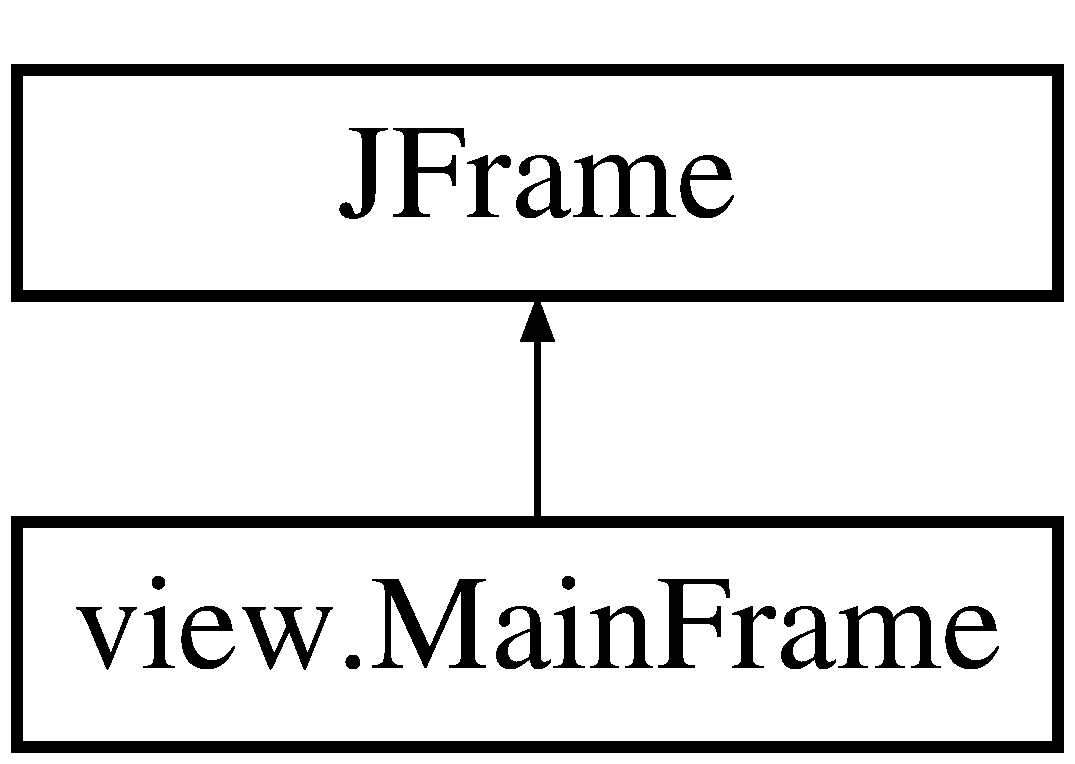
\includegraphics[height=2.000000cm]{classview_1_1_main_frame}
\end{center}
\end{figure}
\subsection*{Public Member Functions}
\begin{DoxyCompactItemize}
\item 
\hypertarget{classview_1_1_main_frame_a6b1386d4f506e5d1ecb4b14e9884ace8}{}\hyperlink{classview_1_1_main_frame_a6b1386d4f506e5d1ecb4b14e9884ace8}{Main\+Frame} ()\label{classview_1_1_main_frame_a6b1386d4f506e5d1ecb4b14e9884ace8}

\begin{DoxyCompactList}\small\item\em Konstruktor. Egy gombot jelenit meg, melynek hatasara kirajzolodik a palya. \end{DoxyCompactList}\end{DoxyCompactItemize}


\subsection{Detailed Description}
A jatek megjelniteset vegzo osztaly. 

\begin{DoxyAuthor}{Author}
team05 
\end{DoxyAuthor}


The documentation for this class was generated from the following file\+:\begin{DoxyCompactItemize}
\item 
C\+:/\+Users/Ádám/\+Desktop/2/checkers/src/view/Main\+Frame.\+java\end{DoxyCompactItemize}

\hypertarget{classmodel_1_1_pair}{}\section{model.\+Pair Class Reference}
\label{classmodel_1_1_pair}\index{model.\+Pair@{model.\+Pair}}


Egy int (x,y) parost reprezentalo osztaly.  


\subsection*{Public Member Functions}
\begin{DoxyCompactItemize}
\item 
\hyperlink{classmodel_1_1_pair_a5d9682977b807703331548d1d4eebfc2}{Pair} (int x, int y)
\item 
int \hyperlink{classmodel_1_1_pair_af525b0d813e70888261660df597cca69}{get\+X} ()
\begin{DoxyCompactList}\small\item\em Visszaadja az X koordinatat. \end{DoxyCompactList}\item 
int \hyperlink{classmodel_1_1_pair_a0da9fc675ede9db0ffce18a8eb586894}{get\+Y} ()
\begin{DoxyCompactList}\small\item\em Visszaadja az Y koordinatat. \end{DoxyCompactList}\end{DoxyCompactItemize}


\subsection{Detailed Description}
Egy int (x,y) parost reprezentalo osztaly. 

\begin{DoxyAuthor}{Author}
team05 
\end{DoxyAuthor}


\subsection{Constructor \& Destructor Documentation}
\hypertarget{classmodel_1_1_pair_a5d9682977b807703331548d1d4eebfc2}{}\index{model\+::\+Pair@{model\+::\+Pair}!Pair@{Pair}}
\index{Pair@{Pair}!model\+::\+Pair@{model\+::\+Pair}}
\subsubsection[{Pair}]{\setlength{\rightskip}{0pt plus 5cm}model.\+Pair.\+Pair (
\begin{DoxyParamCaption}
\item[{int}]{x, }
\item[{int}]{y}
\end{DoxyParamCaption}
)}\label{classmodel_1_1_pair_a5d9682977b807703331548d1d4eebfc2}

\begin{DoxyParams}{Parameters}
{\em x} & \\
\hline
{\em y} & Konstruktor \\
\hline
\end{DoxyParams}


\subsection{Member Function Documentation}
\hypertarget{classmodel_1_1_pair_af525b0d813e70888261660df597cca69}{}\index{model\+::\+Pair@{model\+::\+Pair}!get\+X@{get\+X}}
\index{get\+X@{get\+X}!model\+::\+Pair@{model\+::\+Pair}}
\subsubsection[{get\+X}]{\setlength{\rightskip}{0pt plus 5cm}int model.\+Pair.\+get\+X (
\begin{DoxyParamCaption}
{}
\end{DoxyParamCaption}
)}\label{classmodel_1_1_pair_af525b0d813e70888261660df597cca69}


Visszaadja az X koordinatat. 

\begin{DoxyReturn}{Returns}
int 
\end{DoxyReturn}
\hypertarget{classmodel_1_1_pair_a0da9fc675ede9db0ffce18a8eb586894}{}\index{model\+::\+Pair@{model\+::\+Pair}!get\+Y@{get\+Y}}
\index{get\+Y@{get\+Y}!model\+::\+Pair@{model\+::\+Pair}}
\subsubsection[{get\+Y}]{\setlength{\rightskip}{0pt plus 5cm}int model.\+Pair.\+get\+Y (
\begin{DoxyParamCaption}
{}
\end{DoxyParamCaption}
)}\label{classmodel_1_1_pair_a0da9fc675ede9db0ffce18a8eb586894}


Visszaadja az Y koordinatat. 

\begin{DoxyReturn}{Returns}
int 
\end{DoxyReturn}


The documentation for this class was generated from the following file\+:\begin{DoxyCompactItemize}
\item 
C\+:/\+Users/Ádám/\+Desktop/2/checkers/src/model/Pair.\+java\end{DoxyCompactItemize}

\hypertarget{classmodel_1_1_queen2}{}\section{model.\+Queen2 Class Reference}
\label{classmodel_1_1_queen2}\index{model.\+Queen2@{model.\+Queen2}}


A kirajnot (damat) reprezentalo osztaly.  


Inheritance diagram for model.\+Queen2\+:\begin{figure}[H]
\begin{center}
\leavevmode
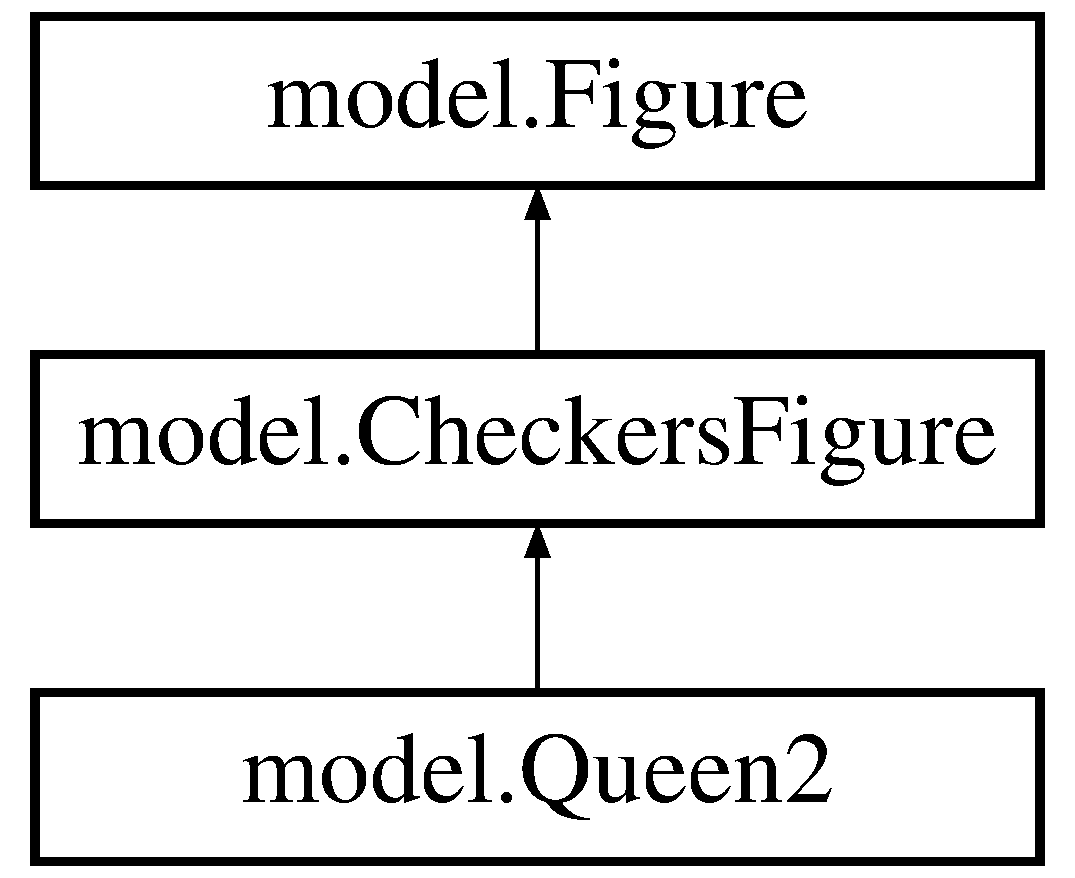
\includegraphics[height=3.000000cm]{classmodel_1_1_queen2}
\end{center}
\end{figure}
\subsection*{Public Member Functions}
\begin{DoxyCompactItemize}
\item 
\hyperlink{classmodel_1_1_queen2_a789867bf846c7ea756dff018e38fe5db}{Queen2} (int pos\+X, int pos\+Y, boolean dark)
\begin{DoxyCompactList}\small\item\em Konstruktor. \end{DoxyCompactList}\item 
boolean \hyperlink{classmodel_1_1_queen2_af7caf10d17bb953cf310f17c2ace0ccf}{can\+Move\+To} (int x, int y)
\begin{DoxyCompactList}\small\item\em Visszaadja, hogy a parameterul kapott koordinatakra lephet-\/e a babu. \end{DoxyCompactList}\end{DoxyCompactItemize}


\subsection{Detailed Description}
A kirajnot (damat) reprezentalo osztaly. 

\begin{DoxyAuthor}{Author}
team05 
\end{DoxyAuthor}


\subsection{Constructor \& Destructor Documentation}
\hypertarget{classmodel_1_1_queen2_a789867bf846c7ea756dff018e38fe5db}{}\index{model\+::\+Queen2@{model\+::\+Queen2}!Queen2@{Queen2}}
\index{Queen2@{Queen2}!model\+::\+Queen2@{model\+::\+Queen2}}
\subsubsection[{Queen2}]{\setlength{\rightskip}{0pt plus 5cm}model.\+Queen2.\+Queen2 (
\begin{DoxyParamCaption}
\item[{int}]{pos\+X, }
\item[{int}]{pos\+Y, }
\item[{boolean}]{dark}
\end{DoxyParamCaption}
)}\label{classmodel_1_1_queen2_a789867bf846c7ea756dff018e38fe5db}


Konstruktor. 


\begin{DoxyParams}{Parameters}
{\em pos\+X} & \\
\hline
{\em pos\+Y} & \\
\hline
{\em dark} & \\
\hline
\end{DoxyParams}


\subsection{Member Function Documentation}
\hypertarget{classmodel_1_1_queen2_af7caf10d17bb953cf310f17c2ace0ccf}{}\index{model\+::\+Queen2@{model\+::\+Queen2}!can\+Move\+To@{can\+Move\+To}}
\index{can\+Move\+To@{can\+Move\+To}!model\+::\+Queen2@{model\+::\+Queen2}}
\subsubsection[{can\+Move\+To}]{\setlength{\rightskip}{0pt plus 5cm}boolean model.\+Queen2.\+can\+Move\+To (
\begin{DoxyParamCaption}
\item[{int}]{x, }
\item[{int}]{y}
\end{DoxyParamCaption}
)}\label{classmodel_1_1_queen2_af7caf10d17bb953cf310f17c2ace0ccf}


Visszaadja, hogy a parameterul kapott koordinatakra lephet-\/e a babu. 


\begin{DoxyParams}{Parameters}
{\em x} & \\
\hline
{\em y} & \\
\hline
\end{DoxyParams}
\begin{DoxyReturn}{Returns}
boolean 
\end{DoxyReturn}


The documentation for this class was generated from the following file\+:\begin{DoxyCompactItemize}
\item 
C\+:/\+Users/Ádám/\+Desktop/2/checkers/src/model/Queen2.\+java\end{DoxyCompactItemize}

\hypertarget{classmodel_1_1_stone}{}\section{model.\+Stone Class Reference}
\label{classmodel_1_1_stone}\index{model.\+Stone@{model.\+Stone}}


A jatek alapfigurajat reprezentalo osztaly.  


Inheritance diagram for model.\+Stone\+:\begin{figure}[H]
\begin{center}
\leavevmode
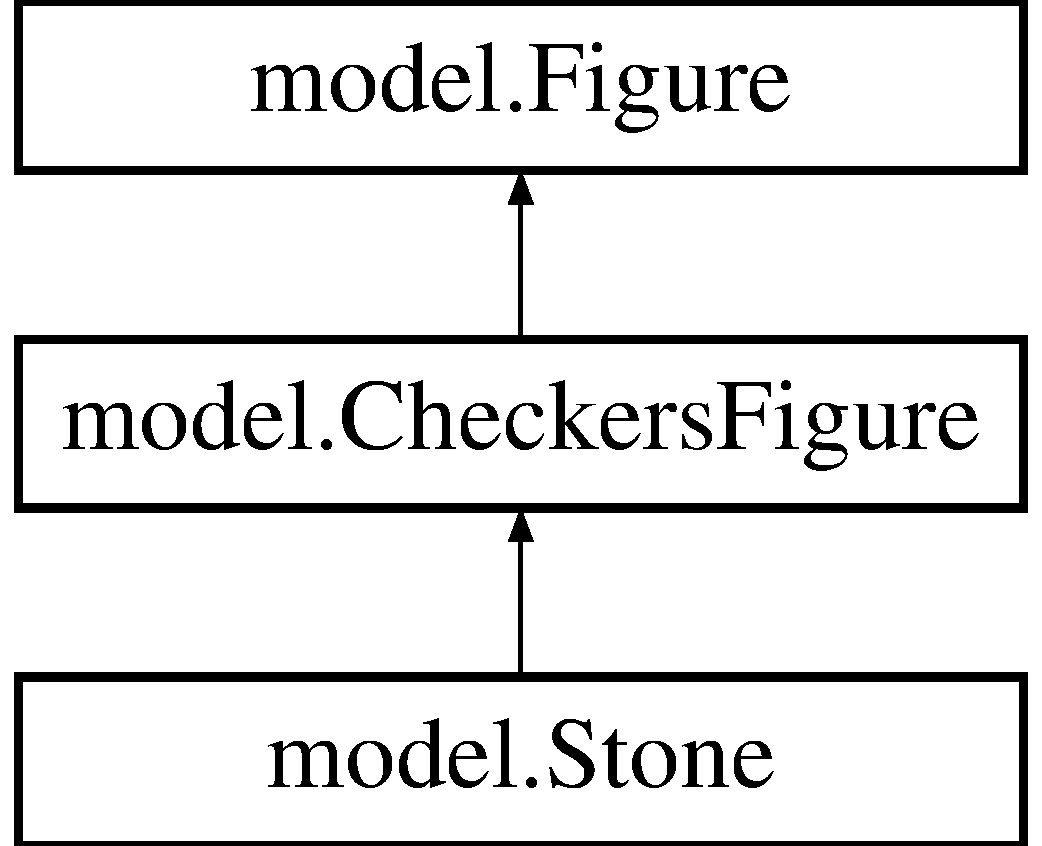
\includegraphics[height=3.000000cm]{classmodel_1_1_stone}
\end{center}
\end{figure}
\subsection*{Public Member Functions}
\begin{DoxyCompactItemize}
\item 
\hyperlink{classmodel_1_1_stone_a73a42818e49280115f8eff4cf69a0d42}{Stone} (int pos\+X, int pos\+Y, boolean dark)
\begin{DoxyCompactList}\small\item\em Konstruktor. \end{DoxyCompactList}\item 
boolean \hyperlink{classmodel_1_1_stone_acf7437d0cba983b4f016c1d0f2decf1b}{can\+Move\+To} (int x, int y)
\begin{DoxyCompactList}\small\item\em Visszaadja, hogy a parameterul kapott koordinatakra tud-\/e lepni a babu. \end{DoxyCompactList}\end{DoxyCompactItemize}


\subsection{Detailed Description}
A jatek alapfigurajat reprezentalo osztaly. 

\begin{DoxyAuthor}{Author}
team05 
\end{DoxyAuthor}


\subsection{Constructor \& Destructor Documentation}
\hypertarget{classmodel_1_1_stone_a73a42818e49280115f8eff4cf69a0d42}{}\index{model\+::\+Stone@{model\+::\+Stone}!Stone@{Stone}}
\index{Stone@{Stone}!model\+::\+Stone@{model\+::\+Stone}}
\subsubsection[{Stone}]{\setlength{\rightskip}{0pt plus 5cm}model.\+Stone.\+Stone (
\begin{DoxyParamCaption}
\item[{int}]{pos\+X, }
\item[{int}]{pos\+Y, }
\item[{boolean}]{dark}
\end{DoxyParamCaption}
)}\label{classmodel_1_1_stone_a73a42818e49280115f8eff4cf69a0d42}


Konstruktor. 


\begin{DoxyParams}{Parameters}
{\em pos\+X} & \\
\hline
{\em pos\+Y} & \\
\hline
{\em dark} & \\
\hline
\end{DoxyParams}


\subsection{Member Function Documentation}
\hypertarget{classmodel_1_1_stone_acf7437d0cba983b4f016c1d0f2decf1b}{}\index{model\+::\+Stone@{model\+::\+Stone}!can\+Move\+To@{can\+Move\+To}}
\index{can\+Move\+To@{can\+Move\+To}!model\+::\+Stone@{model\+::\+Stone}}
\subsubsection[{can\+Move\+To}]{\setlength{\rightskip}{0pt plus 5cm}boolean model.\+Stone.\+can\+Move\+To (
\begin{DoxyParamCaption}
\item[{int}]{x, }
\item[{int}]{y}
\end{DoxyParamCaption}
)}\label{classmodel_1_1_stone_acf7437d0cba983b4f016c1d0f2decf1b}


Visszaadja, hogy a parameterul kapott koordinatakra tud-\/e lepni a babu. 


\begin{DoxyParams}{Parameters}
{\em x} & \\
\hline
{\em y} & \\
\hline
\end{DoxyParams}
\begin{DoxyReturn}{Returns}
boolean 
\end{DoxyReturn}


The documentation for this class was generated from the following file\+:\begin{DoxyCompactItemize}
\item 
C\+:/\+Users/Ádám/\+Desktop/2/checkers/src/model/Stone.\+java\end{DoxyCompactItemize}

\hypertarget{class_checkers_1_1_test_default_colors}{}\section{Checkers.\+Test\+Default\+Colors Class Reference}
\label{class_checkers_1_1_test_default_colors}\index{Checkers.\+Test\+Default\+Colors@{Checkers.\+Test\+Default\+Colors}}


A tabla felrakasat tesztelo osztaly.  


\subsection*{Public Member Functions}
\begin{DoxyCompactItemize}
\item 
\hypertarget{class_checkers_1_1_test_default_colors_aba9afc49712767a0d56b54725f153b2f}{}void {\bfseries test\+Default\+Figures\+Color} ()\label{class_checkers_1_1_test_default_colors_aba9afc49712767a0d56b54725f153b2f}

\item 
\hypertarget{class_checkers_1_1_test_default_colors_aee9bbc2b737677e0dd4d6918c3b2d7fd}{}void {\bfseries set\+Up} ()\label{class_checkers_1_1_test_default_colors_aee9bbc2b737677e0dd4d6918c3b2d7fd}

\item 
\hypertarget{class_checkers_1_1_test_default_colors_a0f6c27514da3c622a9402780a08878a8}{}void {\bfseries tear\+Down} ()\label{class_checkers_1_1_test_default_colors_a0f6c27514da3c622a9402780a08878a8}

\end{DoxyCompactItemize}
\subsection*{Static Public Member Functions}
\begin{DoxyCompactItemize}
\item 
\hypertarget{class_checkers_1_1_test_default_colors_a4d4cf5789a98c263883675826a54d3a3}{}static void {\bfseries set\+Up\+Class} ()\label{class_checkers_1_1_test_default_colors_a4d4cf5789a98c263883675826a54d3a3}

\item 
\hypertarget{class_checkers_1_1_test_default_colors_aae8651d3f1c679af8209d7349bb0b7ff}{}static void {\bfseries tear\+Down\+Class} ()\label{class_checkers_1_1_test_default_colors_aae8651d3f1c679af8209d7349bb0b7ff}

\end{DoxyCompactItemize}


\subsection{Detailed Description}
A tabla felrakasat tesztelo osztaly. 

\begin{DoxyAuthor}{Author}
team05 
\end{DoxyAuthor}


The documentation for this class was generated from the following file\+:\begin{DoxyCompactItemize}
\item 
C\+:/\+Users/Ádám/\+Desktop/2/checkers/test/\+Checkers/Test\+Default\+Colors.\+java\end{DoxyCompactItemize}

\hypertarget{class_checkers_1_1_test_default_places}{}\section{Checkers.\+Test\+Default\+Places Class Reference}
\label{class_checkers_1_1_test_default_places}\index{Checkers.\+Test\+Default\+Places@{Checkers.\+Test\+Default\+Places}}


Az alapjatekosokat es azok felrakasat tesztelo osztaly.  


\subsection*{Public Member Functions}
\begin{DoxyCompactItemize}
\item 
\hypertarget{class_checkers_1_1_test_default_places_ae6eecff89e3b78e7c9935909043fc3ce}{}void {\bfseries test\+Default\+Figures\+Place} ()\label{class_checkers_1_1_test_default_places_ae6eecff89e3b78e7c9935909043fc3ce}

\item 
\hypertarget{class_checkers_1_1_test_default_places_aa9256b3a6b00f5d4fd5c948c4f4b4418}{}void {\bfseries set\+Up} ()\label{class_checkers_1_1_test_default_places_aa9256b3a6b00f5d4fd5c948c4f4b4418}

\item 
\hypertarget{class_checkers_1_1_test_default_places_a644b360d749015b96cd44be4af22394b}{}void {\bfseries tear\+Down} ()\label{class_checkers_1_1_test_default_places_a644b360d749015b96cd44be4af22394b}

\end{DoxyCompactItemize}
\subsection*{Static Public Member Functions}
\begin{DoxyCompactItemize}
\item 
\hypertarget{class_checkers_1_1_test_default_places_af20e2f39313d1c85dcfb74210dd29354}{}static void {\bfseries set\+Up\+Class} ()\label{class_checkers_1_1_test_default_places_af20e2f39313d1c85dcfb74210dd29354}

\item 
\hypertarget{class_checkers_1_1_test_default_places_a6f752a164a2e42e8568b39e9263cfd55}{}static void {\bfseries tear\+Down\+Class} ()\label{class_checkers_1_1_test_default_places_a6f752a164a2e42e8568b39e9263cfd55}

\end{DoxyCompactItemize}


\subsection{Detailed Description}
Az alapjatekosokat es azok felrakasat tesztelo osztaly. 

\begin{DoxyAuthor}{Author}
team05 
\end{DoxyAuthor}


The documentation for this class was generated from the following file\+:\begin{DoxyCompactItemize}
\item 
C\+:/\+Users/Ádám/\+Desktop/2/checkers/test/\+Checkers/Test\+Default\+Places.\+java\end{DoxyCompactItemize}

%--- End generated contents ---

% Index
\backmatter
\newpage
\phantomsection
\clearemptydoublepage
\addcontentsline{toc}{chapter}{Index}
\printindex

\end{document}
